

\documentclass[12pt]{article}
\usepackage[T1]{fontenc}
\usepackage[a4paper, total={7in, 10in}]{geometry}
\usepackage{graphicx}
\usepackage[export]{adjustbox}
\usepackage[font=normalsize,labelfont=bf]{caption}
\usepackage{caption}
\usepackage{amsmath}
\usepackage{subcaption}
\usepackage{float}
\usepackage{titling}
\usepackage{fancyhdr}
\usepackage{lipsum}
\usepackage{amsmath}
\usepackage{siunitx} % For SI unit formatting
\usepackage{booktabs}
\usepackage{tabularx}
\usepackage{textcomp}
\usepackage[polish]{babel}
\usepackage[hidelinks]{hyperref}
\newcommand{\mytitle}{\textbf{BADANIE STANU NAPRĘŻENIA W CIENKOŚCIENNEJ POWŁOCE ZBIORNIKA CIŚNIENIOWEGO}}
\newcommand{\mysubtitle}{Propozycja modernizacji aparatury pomiarowej wykorzystywanej\\ w ramach ćwiczenia nr 9 na zajęciach z przedmiotu \\Laboraturium Podstaw Konstrukcji Maszyn}
\newcommand{\me}{Mateusz Klisiewicz}
\fancyfoot{}
\fancyhead[R]{\me}
\fancyhead[L]{Modernizacja LAB PKM Ćw 9}

\fancyfoot[C]{\thepage}

\renewcommand\maketitlehooka{\null\mbox{}\vfill}
\renewcommand\maketitlehookd{\vfill\null}
\renewcommand{\figurename}{Rysunek}
\renewcommand{\tablename}{Tabela}
\graphicspath{{./res/}}
\title{\mytitle \\
	\large \mysubtitle}
\author{\me}
\date{\today}

\begin{document}
	\pagestyle{fancy}
	\maketitle
	\newpage
\section{Wstęp}
	Przedmiotem badań Ćwiczenia nr 9 jest określenie i analiza rozkładu naprężeń w powłoce cienkościennego zbiornika, obciążonego ciśnieniem wewnętrznym. Zgodnie z instrukcją $^{\cite{manual}}$, ćwiczenie stawia sobie za cel również poznanie komputerowego systemu służącego do rejestracji i obróbki danych. \\
	W obecnej postaci, zajęcia te sprowadzają się do treningu koordynacji ręka-oko, poprzez naciskanie przycisku w "specjalnie opracowanym programie", w zależności od bieżącego ciśnienia w zbiorniku, wyświetlanego na wyświetlaczu enigmatycznego "wzmacniacza typu CL100". W ten sposób studenci uzyskują gotowe zestawy danych, z których następnie tworzą wykresy w programie MS Excel 97 i na tej podstawie sporządzają sprawozdanie.\\
	Sposób w jaki została przygotowana obecna instrukcja do ćwiczenia sprawia, że studenci nie wnioskują samodzielnie w kwestii rozkładu naprężeń, a jedynie porównują kształt otrzymanych wykresów z wykresami opisanymi w instrukcji, by następnie przeformułować wnioski autora i bezrefleksyjnie umieścić je w sprawozdaniu. Takie podejście do zajęć jest wtórne, nie poszerza w istotny sposób wiedzy studentów w zakresie realizacji badań laboratoryjnych, a tym bardziej nie skłania do próby zrozumienia badanego zjawiska. Główny cel ćwiczenia nie jest więc spełniony, a przestarzała aparatura i jej nadmiarowe skomplikowanie sprawiają, że studenci nie są w stanie zapoznać się z nowoczesnymi metodami pomiaru i analizy danych.\\\\
	Biorąc pod uwagę fakt, że przedmiot jest realizowany w ramach kierunku Mechanika Pojazdów i Maszyn Roboczych, zrozumiałym jest pominięcie zawiłych szczegółów, dotyczących konstrukcji układu elektronicznego odczytującego i przetwarzającego niezbędne dane.\\
	Niemniej jednak, cała aparatura jest przeskalowana, i zaprojektowana w sposób nieadekwatny do realizowanych zadań. Zakładając prawdziwość wszystkich danych zawartych w instrukcji, zauważa się użycie "wzmacniacza prądu stałego typu CL100", przez co rozumie się wykorzystanie produktu, który "przeznaczony jest do pracy w szczególnie trudnych warunkach	klimatycznych i mechanicznych. Zalecany jest do stosowania w przemyśle i wszędzie tam, gdzie
	wymagana jest duża odporność na zapylenie i wibracje oraz niezbędna jest bryzgoszczelność." $^{\cite{cl100}}$, a więc urządzenia przemysłowego, spełniającego najróżniejsze normy szczelności i wytrzymałości, które są zupełnie zbędne w warunkach laboratoryjnych. Ponadto zaznaczony jest fakt wykorzystania niezwykle trudno dostępnych i kosztownych tensometrów firmy Vishay. Wnioskuje się użycie tensometrów foliowych, których dokumentacja dostępna jest na stronie firmy związanej z Vishay$^{\cite{tenso}\cite{tenso2}}$ i nie wykazuje żadnych szczególnych właściwości dostępnych modeli, za to odwołuje się do ciężkiej do znalezienia dokumentacji serii tensometrów, co może budzić pewne wątpliwości co do zasadności skorzystania z czujników tej firmy. Co więcej, instrukcja nie informuje o kompensacji temperaturowej pomiarów naprężeń, a producent wzmacniacza deklaruje, że jest on przeznaczony do współpracy "z czujnikami tensometrycznymi \textit{z tensometrami w układzie pełnego mostka}", co dalej podważa zasadność wykorzystania tak drogich komponentów.\\\\
	Niniejszy dokument jest propozycją przeprojektowania aparatury, będącą częścią kompleksowej modernizacji laboratoriów na wydziale Samochodów i Maszyn Roboczych. Głównym obiektem zainteresowania będzie zmiana sposobu odczytu wartości tensometrów, mierzących naprężenia w powłoce zbiornika, oraz sposobu interakcji studentów z urządzeniem. Celem projektu jest przystosowanie aparatury pomiarowej do nowoczesnych standardów, jednocześnie utrzymując jak najniższe koszty przebudowania układu. Tym sposobem chce się uzyskać większe zaangażowanie studentów, poprzez zmuszenie użytkownika do zrozumienia badanego zjawiska przed przystąpieniem do eksperymentu, oraz wyeliminowanie komicznego efektu zabytkowych urządzeń elektronicznych na największej uczelni technicznej w Polsce.\\ Docelowo planuje się ustandaryzowany system komunikacji ze stanowiskami pomiarowymi poprzez ogólnodostępną, wydziałową aplikację laboratoryjną, oferującą możliwość prowadzenia niezależnych symulacji zjawisk, prezentowanych na zajęciach na uczelni. Jednocześnie uwzględnia się konieczność możliwości przeprowadzenia dowolnego eksperymentu lokalnie, na komputerze powiązanym ze stanowiskiem.
	
\section{Założenia}
	Podczas projektowania układu zakłada się co następuje:
	\begin{enumerate}
		\item[1] Preferencje korzystania z budżetowych rozwiązań, jednocześnie nie rezygnując z dokładności pomiarów
		\item[2] Sprawność tensometrów wykorzystywanych w obecnej aparaturze
		\item[3] Odkształcenia tensometrów w zakresie $0.0-0.1 \% $
		\item[4] Przez 32 tensometry opisane w instrukcji ćwiczenia rozumie się 64 tensometry pracujące w układzie 32 półmostków typu I$^{\cite{gages}}$, naklejone w pomijalnej odległości parami, lub jako pary pojedynczych elementów zintegrowanych, tworzące dwa zestawy 16 punktów pomiarowych dla naprężeń promieniowych i obwodowych
		\item[5] Tensometry przy braku obciążenia charakteryzują się rezystancją $R_0=350\Omega$, długością\\ $l_0=3mm$ oraz stałą tensometru $GF=2.15$ typową dla podobnych komponentów, przyjętą  ze względu na brak informacji w karcie produktu$^{\cite{tenso}}$
		\item[6] Badany zbiornik wykonany jest ze stali 1.4541 (1H18N9T) charakteryzującej się współczynnikiem Poisson'a $\nu = 0.28^{\cite{steel}}$
		\item[7] System sterowany będzie przez układ scalony RP2040 i jego implementację w płytce rozwojowej Raspberry Pi Pico, co ustala poziom logiczny i napięcie zasilania komponentów składowych $U_l = 3.3V$
	\end{enumerate}
	
	\begin{figure}[H]
		\centering
		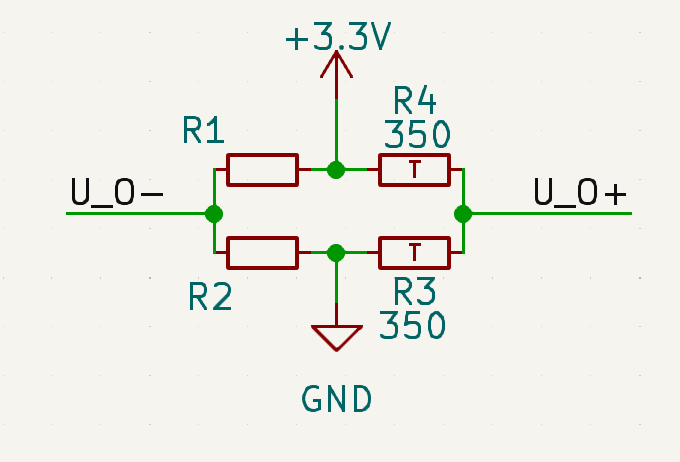
\includegraphics[width=0.4\textwidth, center]{half_bridge}
		\caption{Półmostek Wheatstone'a typu I, gdzie: $R_3, R_4$ - wartości rezystancji tensometrów, $R_1, R_2$ - rezystory o odpowiednio ustalonej rezystancji}
		\label{rys:bridge}
	\end{figure}
	
	Wykorzystywane półmostki charakteryzują się użyciem dwóch rezystorów o ustalonych wartościach $R_1, R_2$ oraz dwóch tensometrów $R_3, R_4$, z których $R_4$ jest tensometrem głównym, poddawanym mierzonemu naprężeniu, natomiast $R_3$ jest tensometrem kompensującym efekt Poisson'a$^{\cite{gages2}}$ poddawany naprężeniom w osi prostopadłej do osi naprężeń mierzonych.\\
	Dla mostka tego typu zachodzi zależność:
	\begin{equation}
		U_0 = U_{0+} - U_{0-} = U_l \cdot \left(\frac{R_3}{R_3+R_4}- \frac{R_2}{R_1+R_2}\right),
	\end{equation}
	oraz dla sytuacji, w której tensometry nie są obciążone:
	\begin{equation}
		\frac{R_1}{R_2}=\frac{R_{04}}{R_{03}},
	\end{equation}
	Zgodnie z powyższymi założeniami oraz zależnością $^{\cite{gages}}$:
	\begin{align*}
		GF&=\frac{\frac{\Delta R}{R_4}}{\frac{\Delta l}{l_0}}=\frac{\frac{\Delta R}{R_4}}{\varepsilon},\\
		\varepsilon &= \frac{\frac{\Delta R}{R_4}}{GF}
	\end{align*}
	przy czym, dla tensometru kompensującego zachodzi:
	\begin{align*}
		GF&=\frac{\frac{\Delta R}{R_3}}{\frac{\Delta l}{l_0}}=\frac{\frac{\Delta R}{R_3}}{-\nu \varepsilon},\\
		-\nu \varepsilon &= \frac{\frac{\Delta R}{R_3}}{GF},
	\end{align*}
	zakładając:
	\begin{equation}
		R_1 = R_2 = R_{03} = R_{04} = R_T = 350\Omega,
	\end{equation}
	otrzymuje się:
	\begin{equation}
		\varepsilon = \frac{-4U_r}{GF[(1+\nu)-2U_r(\nu-1)]},
	\end{equation}
	gdzie $U_r = \frac{U_0}{U_l}$.\\
	Przyjmując według założeń:
	\begin{align}
		\frac{\Delta l_{max}}{l_0} &= \varepsilon_{max} = 0.001,
	\end{align}
	można wyznaczyć najwyższe mierzone napięcie na wyjściu mostka:
	\begin{align}
		U_{0max} &= \frac{\varepsilon_{max}GF(1+\nu)}{4-2\varepsilon_{max} GF(\nu-1)}U_l \approx 0.0022686V,\\
		U_{0max} &= 2268.6\mu V
	\end{align}
	
	 
\section{Proponowane Rozwiązanie}

	Na podstawie powyższych rozważań wnioskuje się, że zachodzi konieczność pomiaru 32 kanałów różnicowych, z dokładnością rzędu $1 - 10\mu V$ dla zadowalającej rozdzielczości. Rezygnuje się ze zwiększenia napięcia zasilania mostków w celu zwiększenia wartości mierzonych napięcia, z powodu braku kompensacji temperaturowej i wysokiej wrażliwości danych tensometrów.\\
	Ze względu na wysokie koszty wielokanałowych przetworników analogowo-cyfrowych proponuje się zastosowanie dwóch multiplekserów różnicowych w konfiguracji 16:1, po jednym na zestaw mostków. W ten sposób redukuje się ilość kanałów różnicowych do 2 co pozwala zastosować mniejszy i tańszy przetwornik, kosztem konieczności kompensacji dodatkowej rezystancji oraz wydłużenia czasu pojedynczego pomiaru do około 1ms$^{\cite{multi}}$ wynikającego z czasu przełączania 16 źródeł. Wpływ czasu pomiaru na jakość otrzymanych danych zależy od wydajności pompy ciśnienia, jednak przy mierzonych wartościach wydaje się nie mieć istotnego znaczenia. Takie podejście pozwala zastosować 2-kanałowy 24-bitowy przetwornik analogowo-cyfrowy np. ADS131M02$^{\cite{adc}}$ posiadający możliwość wzmocnienia sygnału 128-krotnie. Przy pożądanej dokładności takie wzmocnienie, wraz z wysoką ilością bitów, pozwala w teorii mierzyć z dokładnością na poziomie $0.002\mu V$, co znacząco przewyższa potrzeby eksperymentu i pozwala pominąć wzmacniacz instrumentalny przed kanałem przetwornika. Analogiczne rozwiązanie można zastosować w układzie czujnika ciśnienia całkowicie eliminując obecnie wykorzystywane wzmacniacze i stosując 3- lub 4-kanałowy ADC$^{\cite{adc3}}$ zamiast 2-kanałowego. 
	\subsection{Schemat}
	\begin{figure}[H]
		\centering
		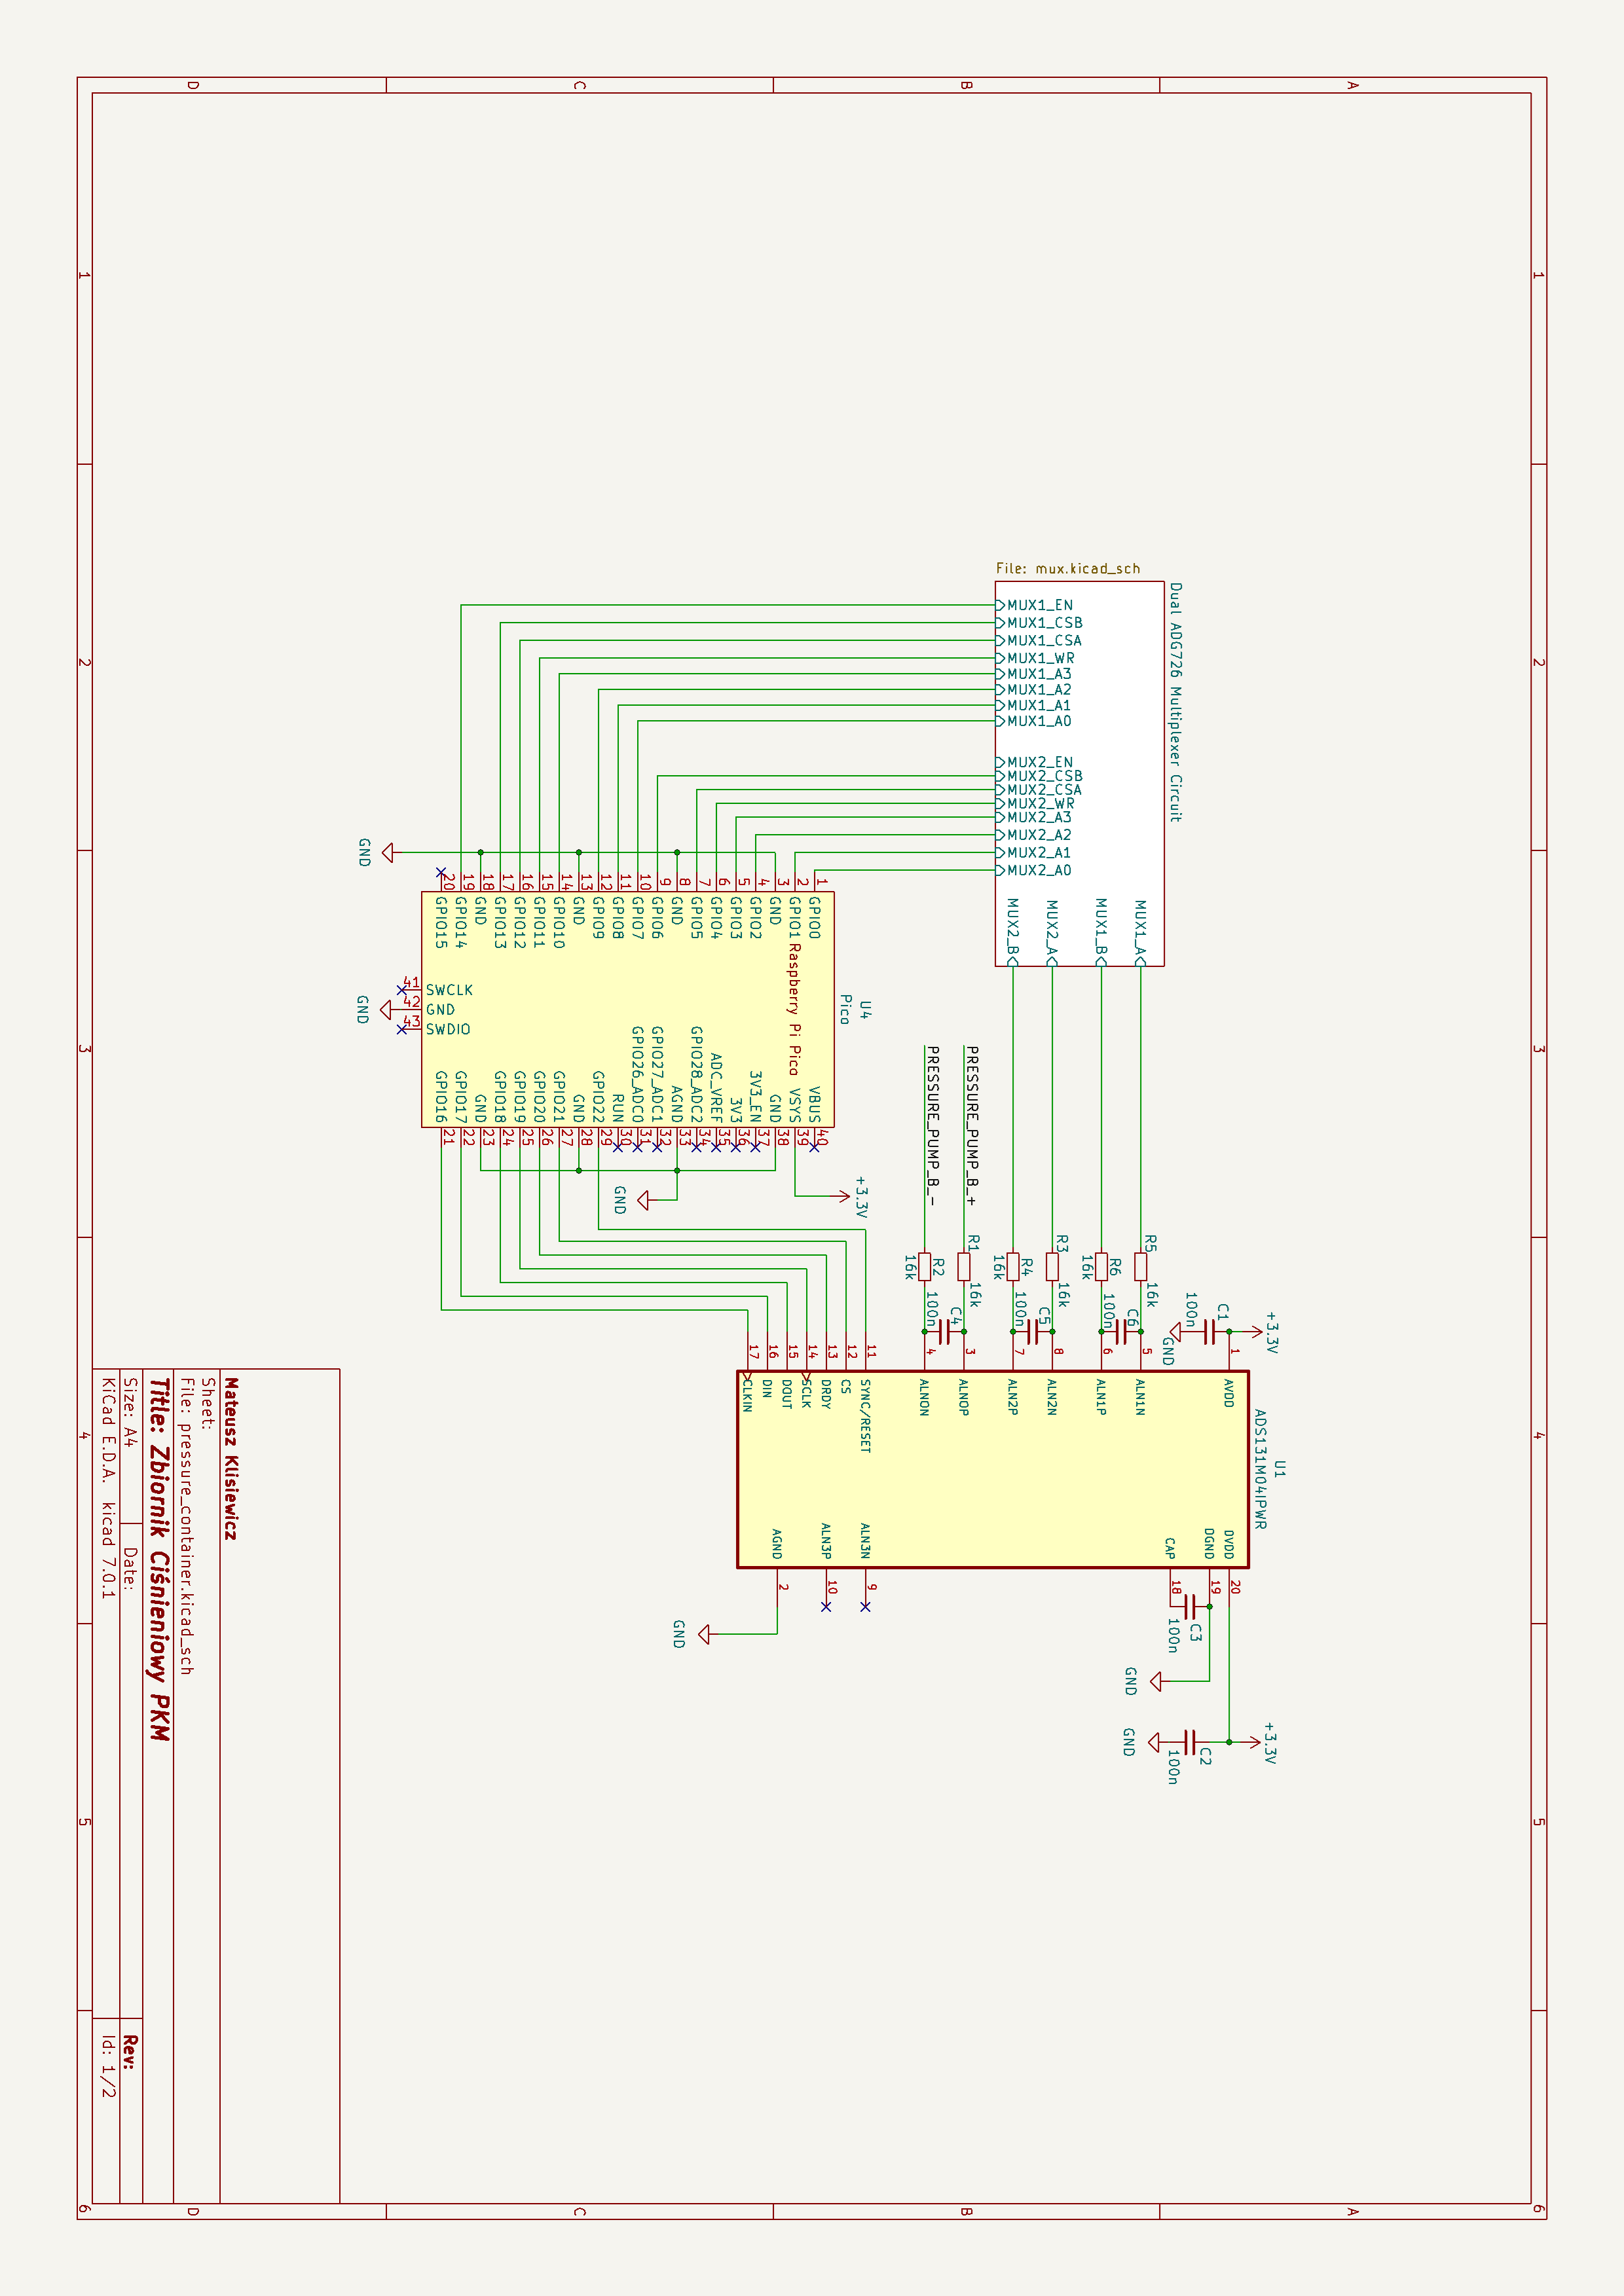
\includegraphics[width=0.75\textwidth, center]{schematic}
		\caption{Przykładowy schemat połączeń układu dwóch multiplekserów ADG726 z konwerterem ADC131M03 i mikrokontrolerem RaspberryPi Pico}
		\label{rys:sch}
	\end{figure}
	\subsection{Przebieg Ćwiczenia}
	Wyżej opisany układ, w połączeniu z odpowiednio przygotowaną aplikacją, pozwala na odczyt wszystkich niezbędnych danych, bezpośrednio z komputera połączonego z mikrokontrolerem poprzez interfejs USB. Szczegółowy przebieg ćwiczenia jest przedmiotem do głębszego omówienia i zależy od pożądanych efektów kształcenia.\\ 
	Proponuje się aby studenci otrzymywali wartości wzmocnionych napięć dla poszczególnych punktów pomiarowych w zależności od naprężenia w zbiorniku. Zakres tych danych oraz skok ciśnienia między poszczególnymi pomiarami mógłby być ustalany w aplikacji komputerowej. Zadaniem użytkowników byłoby przekształcenie wzmocnionych wartości na wartości rzeczywiste, ustalenie na tej podstawie wartości odkształceń względnych oraz sporządzenie wykresów i samodzielne dojście do wniosków zapisanych w obecnej instrukcji.\\
	W nowej instrukcji do ćwiczenia zawarty by był opis aparatury podobny do tego, który przedstawiany jest teraz. Bardziej szcegółowo mogłaby być opisana zasada działania układu wzmacniacza i ADC, z podanymi wartościami wzmocnienia i dokładnością realizowanych pomiarów. Większą uwagę można by było poświęcić teorii wytrzymałości zbiorników walcowych i porównanie naprężeń obwodowych z naprężeniami wzdłużnymi, a następnie sprawdzić przewidywania teoretyczne w odniesieniu do otrzymanych wyników.\\
	Eksperyment przeprowadzony w ten sposób zmuszałby studentów do zapoznania się z zasadą działania czujników tensometrycznych w układzie półmostków, typowymi wartościami napięcia mierzonymi za pomocą takich czujników oraz sposobem interpretacji uzyskanych danych. Ponadto, na podstawie samodzielnie obliczonych wyników, studenci mogliby wnioskować o rozkładzie naprężeń w  cienkościennej powłoce zbiornika ciśnieniowego. Tak przeprowadzone ćwiczenie może służyć jako uzupełnienie (lub wprowadzenie) do ćwiczenia nr 2 (Wyznaczanie naprężeń w rurze prostej). Należy zwrócić uwagę na fakt, że każde z ćwiczeń realizowanych w ramach przedmiotu, polega na tensometrycznym pomiarze odkształceń różnych konstrukcji, jednakże kwestia ta zdaje się nie być wystarczająco podkreślona i objaśniona.
	\subsection{Wstępny Kosztorys} 
	\begin{table}[h!]
		\centering
		\begin{tabularx}{\textwidth}{|c|X|c|c|c|}
			\hline
			\textbf{Produkt} & \textbf{Opis} & \textbf{Cena (PLN)} & \textbf{Ilość} & \textbf{Cena całkowita(PLN)} \\
			\hline
			ADG726BSUZ & Multiplexer Switch ICs 1.8V to 5.5V, D/D 16:1Mux Par I/F I.C. & 58.56$^{\cite{adg726}}$ & 2 & 117.12 \\
			\hline
			ADS131M03IPWR & Analog to Digital Converters - ADC Three-channel, 24-bit, 64-kSPS, simultaneous-sampling, delta-sigma ADC 20-TSSOP -40 to 125 & 18.66$^{\cite{ads131}}$ & 1 & 18.66 \\
			\hline
			Raspberry Pi Pico & Mikrokontroler & 16.26$^{\cite{pico}}$ & 1 & 16.26 \\
			\hline
			Dodatkowe Koszty & Elementy pasywne, regulator napięcia, półprodukty do przygotowania PCB, dostawa & 30 - 40 & 1 & 30 - 40 \\
			\hline
			\multicolumn{4}{|r|}{\textbf{Koszt całkowity}} & \textbf{182.04 - 192.04} \\
			\hline
		\end{tabularx}
		\caption{Kosztorys pomiarowego układu elektronicznego}
		\label{tab:cost_summary}
	\end{table}
	W celu uzyskania jak najlepszej ekonomii modernizacji, należałoby również rozważyć koszty przebudowy innych eksperymentów oraz uwzględnić potrzeby innych zakładów wydziału. Pozwoli to na wyeliminowanie kosztów dostawy produktów oraz zamówienie układów według korzystniejszych cen jednostkowych dla zamówień hurtowych.
	\subsection{Pozostałe Propozycje}
	Należy pamiętać, że powyższa propozycja jest oparta na wstępnych rozważaniach i określonych założeniach. W zależności od potrzeb, możliwa jest redukcja kosztów poprzez zastosowanie innego układu, np. korzystającego z dwóch 16-kanałowych, 16-bitowych przetworników ADC$^{\cite{16adc}}$ z zastosowaniem wzmacniaczy instrumentalnych$^{\cite{amp}}$ redukujących 32 kanały różnicowe do 32 pojedynczych kanałów z odniesieniem do $GND$. Innym podejściem może być zastosowanie konwerterów o mniejszej rozdzielczości wraz z multiplekserami. W celu wybrania odpowiedniego rozwiązania konieczne jest szczegółowe określenie wymagań dotyczących aparatury i przebiegu eksperymentu.
	
\begin{thebibliography}{1}
	\bibitem{manual} \href{./Instrukcja.pdf}{\textit{Benedykt Ponder - Instrukcja cw.9 - zbiornik cisnieniowy 2007}}
	\bibitem {cl100} \href{https://cms.zepwn.com.pl/karty%20pl/elektronika/Karta_CL100P_2018.02.01.pdf}{\textit{Wzmacniacz prądu stałego CL100}}
	\bibitem {tenso}  \href{https://docs.micro-measurements.com/?id=2590}{\textit{General Purpose Strain Gages}}
	\bibitem{tenso2} \href{https://docs.micro-measurements.com/?id=2512}{\textit{General Purpose Strain Gages—Linear Pattern 062UW}}
	\bibitem {gages}  \href{http://elektron.pol.lublin.pl/elekp/ap_notes/ni_an078_strain_gauge_meas.pdf}{\textit{Strain Gauge Measurement – A Tutorial}}
	\bibitem {gages2} \href{https://www.ni.com/en/shop/data-acquisition/sensor-fundamentals/measuring-strain-with-strain-gages.html}{\textit{Measuring Strain with Strain Gages}}
	\bibitem {steel}  \href{https://www.makeitfrom.com/material-properties/EN-1.4541-X6CrNiTi18-10-Stainless-Steel}{\textit{EN1.4541 (X6CrNiTi18-10) Stainless Steel}}
	\bibitem{multi}  \href{https://www.mouser.pl/datasheet/2/609/ADG726_732-1503078.pdf}{\textit{ADG726/ADG732 16-/32-Channel, 4 $\Omega$, +1.8 V to +5.5 V and	±2.5 V Analog Multiplexers}}
	\bibitem{adc} \href{https://www.ti.com/lit/ds/symlink/ads131m02.pdf?ts=1720442471757&ref_url=https%253A%252F%252Fwww.mouser.it%252F}{\textit{ADS131M02 2-Channel, Simultaneously-Sampling, 24-Bit, Delta-Sigma ADC}}
	\bibitem{adc3} \href{https://www.ti.com/lit/ds/symlink/ads131m03.pdf?ts=1720454719799&ref_url=https%253A%252F%252Fwww.mouser.pl%252F}{\textit{ADS131M03 3-Channel, Simultaneously-Sampling, 24-Bit, Delta-Sigma ADC}}
	\bibitem{adc_wiki} \href{https://en.wikipedia.org/wiki/Analog-to-digital_converter}{\textit{Analog-to-digital converter}}
	\bibitem{adg726} \href{https://www.mouser.pl/ProductDetail/Analog-Devices/ADG726BSUZ?qs=BpaRKvA4VqHCQkaid0DsDg%3D%3D}{\textit{ADG726BSUZ }}
	\bibitem{ads131} \href{https://www.mouser.pl/ProductDetail/Texas-Instruments/ADS131M03IPWR?qs=sGAEpiMZZMutXGli8Ay4kK6SD7YYu%252BTeEMXHMz4FMLA%3D}{\textit{ADS131M03IPWR}}
	\bibitem{pico} \href{https://www.mouser.pl/ProductDetail/358-SC0915}{\textit{Raspberry Pi Pico}}
	\bibitem{16adc} \href{https://www.mouser.pl/ProductDetail/Analog-Devices/LTC2497CUHFTRPBF?qs=hVkxg5c3xu%252BLBexp2AEE0A%3D%3D}{\textit{LTC2497CUHF}}
	\bibitem{amp} \href{https://www.mouser.pl/ProductDetail/Texas-Instruments/INA350CDSIDDFR?qs=t7xnP681wgW6%252BiL92FfJng%3D%3D}{\textit{INA350CD}}
	
\end{thebibliography}
\end{document}